\documentclass[convert={density=300,size=1080x800,outext=.png}]{standalone}
\usepackage{tikz}
\usepackage{tikz-network}
\begin{document}
	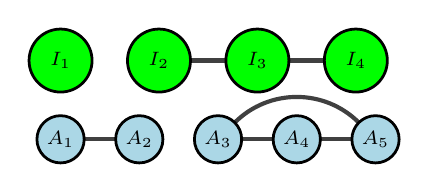
\begin{tikzpicture}

\Vertex[x=0.75,label=$I_1$, color = green, size = .8]{C}
\Vertex[x=2,label=$I_2$,color = green, size = .8]{D}
\Vertex[x=3.25,label=$I_3$,color = green, size = .8]{E}
\Vertex[x=4.5,label=$I_4$,color = green, size = .8]{F}

\Edge(D)(E)
\Edge(E)(F)

\Vertex[x=0.75,y = -1, label=$A_1$, size = .6]{G}
\Vertex[x=1.75,y = -1, label=$A_2$, size = .6]{H}
\Vertex[x=2.75,y = -1, label=$A_3$, size = .6]{I}
\Vertex[x=3.75,y = -1, label=$A_4$, size = .6]{J}
\Vertex[x=4.75,y = -1, label=$A_5$, size = .6]{K}


\Edge(G)(H)
\Edge(I)(J)
\Edge[bend=45](I)(K)
\Edge(J)(K)


\end{tikzpicture}
\end{document}
